% -*- mode: latex; mode: flyspell; ispell-local-dictionary: "en_US"; coding: utf-8; fill-column: 80 -*-

\documentclass{article}

\usepackage[utf8]{inputenc}
\usepackage[english]{babel}

\usepackage{amsmath,amsfonts,amssymb}
\usepackage{fullpage}
\usepackage{verbatim}

\usepackage{tikz,pgfplots}
\usetikzlibrary{patterns, patterns.meta}

\pgfplotsset{
  /pgfplots/bar cycle list/.style = {
    /pgfplots/cycle list = {
      { fill = black!40, mark = none },
      { fill = brown!70, mark = none },
      { fill = blue!70, mark = none },
      { fill = green!60, mark = none },
      { fill = violet!60, mark = none },
      { fill = yellow!90, mark = none },
      { fill = red!60, mark = none },
      { fill = orange!80, mark = none },
    }
  }
}

\pgfplotsset{
  width = 150mm,
  height = 100mm,
  major grid style = { thin, dotted, color = black!50 },
  minor grid style = { thin, dotted, color = black!50 },
  grid,
  xtick distance = 1,
  ymin = 0,
  every axis/.append style = {
    line width = 0.5pt,
    tick style = {
      line cap = round,
      thin,
      major tick length = 4pt,
      minor tick length = 2pt,
    },
  },
  legend cell align = left,
  legend pos = north west,
  enlarge x limits = 0.25,
	/pgfplots/ybar legend/.style = {
		/pgfplots/legend image code/.code={%
			\draw[##1,/tikz/.cd,yshift=-0.25em]
			(0cm,0cm) rectangle (3pt,0.8em);},
	},  
}

\begin{document}

\title{WT Benchmark}
\author{Jan-Philipp Tarnowski}
\maketitle


% IMPORT-DATA stats   results-2022-03-06--11-07-33.out
% IMPORT-DATA stats_b results-2022-03-07--07-47-24.out

% SQL INSERT INTO stats SELECT * FROM stats_b

\begin{center}
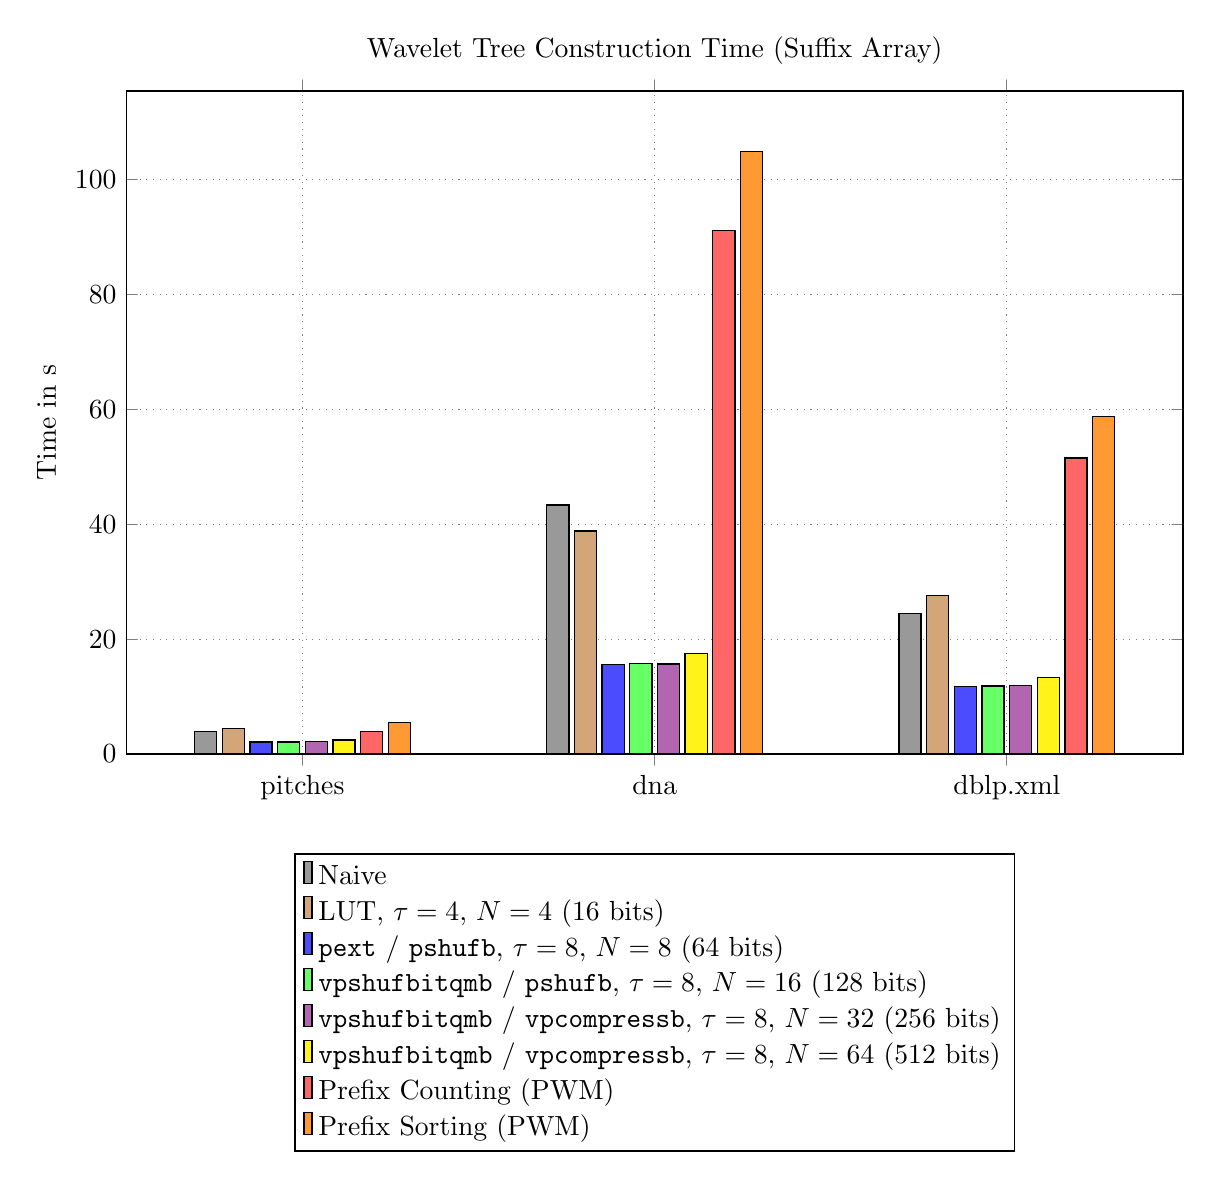
\begin{tikzpicture}
  \begin{axis} [
    ybar,
    bar width = 8pt,
    xtick = data,
    title = {Wavelet Tree Construction Time (Suffix Array)},
    legend style = { at = {(0.5, -0.15)}, anchor = north},
	  ylabel = {Time in s},
    symbolic x coords = {
      pitches,   
      dna,
      dblp.xml
    }
  ]



			%%- MULTIPLOT(type) SELECT file AS x, MEDIAN(time_in_s) AS y,MULTIPLOT 
			%%- FROM stats WHERE (file LIKE 'pitches' OR file LIKE 'dblp.xml' OR file LIKE 'dna') AND (type LIKE 'lwt%' OR type LIKE '%tree') GROUP BY MULTIPLOT,x ORDER BY MULTIPLOT,x
   \addplot coordinates { (dblp.xml,24.4447) (dna,43.3149) (pitches,3.93119) };
   \addlegendentry{type=lwt\_basic};
   \addplot coordinates { (dblp.xml,27.5632) (dna,38.8519) (pitches,4.44851) };
   \addlegendentry{type=lwt\_lut\_4\_4\_1};
   \addplot coordinates { (dblp.xml,11.7713) (dna,15.6056) (pitches,2.08346) };
   \addlegendentry{type=lwt\_pext\_pext\_8};
   \addplot coordinates { (dblp.xml,11.8047) (dna,15.7024) (pitches,2.09597) };
   \addlegendentry{type=lwt\_pext\_pext\_16};
   \addplot coordinates { (dblp.xml,11.9527) (dna,15.6533) (pitches,2.16373) };
   \addlegendentry{type=lwt\_pext\_pext\_32};
   \addplot coordinates { (dblp.xml,13.3171) (dna,17.5222) (pitches,2.41572) };
   \addlegendentry{type=lwt\_pext\_pext\_64};
   \addplot coordinates { (dblp.xml,51.5165) (dna,91.182) (pitches,3.891) };
   \addlegendentry{type=pwm\_5wx\_pcIjLb1EE\_tree};
   \addplot coordinates { (dblp.xml,58.7684) (dna,104.921) (pitches,5.42468) };
   \addlegendentry{type=pwm\_5wx\_psIjLb1EE\_tree};

   \legend{
     Naive \\
     LUT, $\tau = 4$, $N = 4$ (16 bits) \\
     \texttt{pext} / \texttt{pshufb}, $\tau = 8$, $N = 8$ (64 bits) \\
     \texttt{vpshufbitqmb} / \texttt{pshufb}, $\tau = 8$, $N = 16$ (128 bits) \\
     \texttt{vpshufbitqmb} / \texttt{vpcompressb}, $\tau = 8$, $N = 32$ (256 bits) \\
     \texttt{vpshufbitqmb} / \texttt{vpcompressb}, $\tau = 8$, $N = 64$ (512 bits) \\
     Prefix Counting (PWM) \\
     Prefix Sorting (PWM) \\
  };

  \end{axis}
\end{tikzpicture} 
\end{center}

\vspace{1cm}
\begin{tabular}{|lll|}
  \hline
  Text & Size & $\sigma$ \\
  \hline
  pitches & $53.25$ Mib & $132$ \\
  dna & $385.22$ MiB & $16$ \\
  dblp.xml & $282.42$ MiB & $97$ \\
  \hline
\end{tabular}

\pagebreak

  %%%%%%%%%%%%%
  %%%% WM %%%%%
  %%%%%%%%%%%%%

\begin{center}
  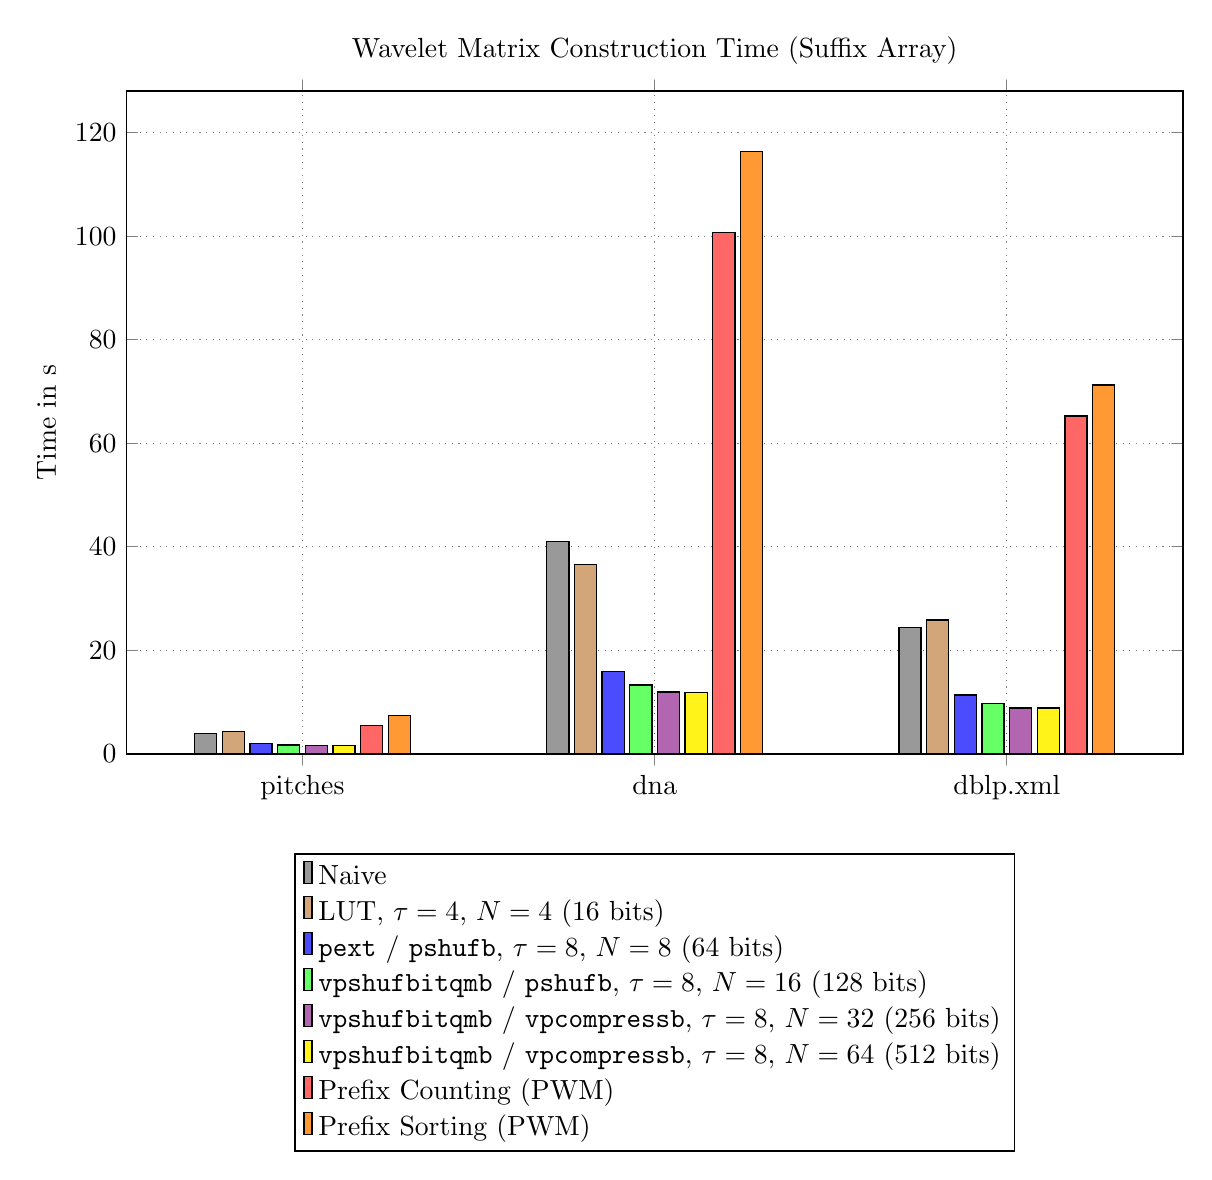
\begin{tikzpicture}
    \begin{axis} [
      ybar,
      bar width = 8pt,
      xtick = data,
      title = {Wavelet Matrix Construction Time (Suffix Array)},
      legend style = { at = {(0.5, -0.15)}, anchor = north},
      ylabel = {Time in s},
      symbolic x coords = {
        pitches,   
        dna,
        dblp.xml
      }
    ]
  
  
  
        %%- MULTIPLOT(type) SELECT file AS x, MEDIAN(time_in_s) AS y,MULTIPLOT 
        %%- FROM stats WHERE (file LIKE 'pitches' OR file LIKE 'dblp.xml' OR file LIKE 'dna') AND (type LIKE 'wm%' OR type LIKE '%matrix') GROUP BY MULTIPLOT,x ORDER BY MULTIPLOT,x
        \addplot coordinates { (dblp.xml,24.4096) (dna,41.0523) (pitches,3.92354) };
        \addlegendentry{type=wm\_basic};
        \addplot coordinates { (dblp.xml,25.8862) (dna,36.5683) (pitches,4.37076) };
        \addlegendentry{type=wm\_lut\_4\_4\_1};
        \addplot coordinates { (dblp.xml,11.3572) (dna,15.9175) (pitches,2.00712) };
        \addlegendentry{type=wm\_pext\_pext\_8};
        \addplot coordinates { (dblp.xml,9.7113) (dna,13.304) (pitches,1.73148) };
        \addlegendentry{type=wm\_pext\_pext\_16};
        \addplot coordinates { (dblp.xml,8.90179) (dna,11.9697) (pitches,1.60745) };
        \addlegendentry{type=wm\_pext\_pext\_32};
        \addplot coordinates { (dblp.xml,8.88307) (dna,11.8784) (pitches,1.57719) };
        \addlegendentry{type=wm\_pext\_pext\_64};
        \addplot coordinates { (dblp.xml,65.3189) (dna,100.701) (pitches,5.46685) };
        \addlegendentry{type=pwm\_5wx\_pcIjLb0EE\_matrix};
        \addplot coordinates { (dblp.xml,71.2638) (dna,116.423) (pitches,7.38547) };
        \addlegendentry{type=pwm\_5wx\_psIjLb0EE\_matrix};

        \legend{
          Naive \\
          LUT, $\tau = 4$, $N = 4$ (16 bits) \\
          \texttt{pext} / \texttt{pshufb}, $\tau = 8$, $N = 8$ (64 bits) \\
          \texttt{vpshufbitqmb} / \texttt{pshufb}, $\tau = 8$, $N = 16$ (128 bits) \\
          \texttt{vpshufbitqmb} / \texttt{vpcompressb}, $\tau = 8$, $N = 32$ (256 bits) \\
          \texttt{vpshufbitqmb} / \texttt{vpcompressb}, $\tau = 8$, $N = 64$ (512 bits) \\
          Prefix Counting (PWM) \\
          Prefix Sorting (PWM) \\
       };
        
  
    \end{axis}
  \end{tikzpicture} 
  \end{center}
  
  \vspace{1cm}
  \begin{tabular}{|lll|}
    \hline
    Text & Size & $\sigma$ \\
    \hline
    pitches & $53.25$ Mib & $132$ \\
    dna & $385.22$ MiB & $16$ \\
    dblp.xml & $282.42$ MiB & $97$ \\
    \hline
  \end{tabular}
  
  \pagebreak
%%%%%%%%%%%%%%%%%%%%%%%%%%%%%%%%%%%%%%%%%%%%%%%%%%%%%%%%%%%%%%%%%%%%%%%%%%%%%%%%

\end{document}
